
\documentclass[twoside,leqno,twocolumn]{article}
\usepackage{ltexpprt}
\usepackage{subfigure}
\usepackage{xcolor}
\usepackage{url}
\usepackage{graphics}
\usepackage{graphicx}
\usepackage{algorithm}
\usepackage{algorithmic}
\usepackage{caption}
\newcommand{\argmin}{\arg\!\min}



\begin{document}
%\setcounter{chapter}{2} % If you are doing your chapter as chapter one,
%\setcounter{section}{3} % comment these two lines out.

\title{Detecting Group Absenteeism in Twitter: Algorithms and Applications}
\author{Fang Jin\thanks{Discovery Analytics Center, Department of Computer Science, Virginia Tech.} \\
\and
Feng Chen\thanks{Department of Computer Science, University at Albany, SUNY.}\\
\and
Chang-Tien Lu\footnotemark[1]\\
\and
Naren Ramakrishnan\footnotemark[1]\\
}
\date{}
\maketitle



%\pagenumbering{arabic}
%\setcounter{page}{1}%Leave this line commented out.

\begin{abstract} \small\baselineskip=9pt Significant attention has been paid to modeling bursts and upticks in social media activity (e.g., Twitter and Facebook shares). An important but unstudied problem is the detection of group absenteeism wherein an unusually low level of activity is observed in a specific spatio-temporal slice of the data. We present the first study to systematically investigate group absenteeism in Twitter. Two practical approaches are developed to detect group absenteeism motivated by different viewpoints. The first approach merges clustering with a rectangle modeling to identify spatially connected dense clusters. The second approach uses a minimum weight subgraph modeling under subgraph diameter constraints. We analyze the strengths and weakness of these two approaches and demonstrate their application to Twitter datasets over Latin America. In particular, we illustrate how the modeling of group absenteeism could shed insight into event detection.\end{abstract}


\section{Introduction.} \label{sec:intro}
Social microblogs such as Twitter and Weibo are experiencing explosive growth, with billions of users globally sharing their daily observations and thoughts online. For example, Twitter has more than 255 million average monthly active users (78\% from mobile) since March 31, 2014 and an estimated increase of 25\% per year\footnote{http://solomozone.com/tag/revenues/}. Various studies have shown that Twitter is viable as a social ``sensor'' and holds great promise for detecting and forecasting of significant societal events~\cite{sakaki2010earthquake, bugel2013multilingual}.

In recent years, the phenomenon of bursts and upticks in social media activity has attracted significant attention~\cite{sakaki2010earthquake, lappas2009burstiness, lappas2012spatiotemporal, yin2011geographical, hong2012discovering, eisenstein2010latent, teitler2008newsstand, weng2011event, sayyadi2009event, watanabe2011jasmine, aggarwal2012event}. The relevant methods can be classified into three categories: burst detection, geographical topic modeling, and clustering. Burst detection methods search for space-time regions that have abnormally high counts of some predefined terms~\cite{lappas2009burstiness, lappas2012spatiotemporal}. Sakaki et al. consider spatial-temporal Kalman filtering to track the geographical trajectories of hot spots of Tweets related to earthquakes~\cite{sakaki2010earthquake}. Geographic topic modeling based methods detect topics of interest that are coherent in geographic regions~\cite{yin2011geographical, hong2012discovering, eisenstein2010latent}. Clustering-based approaches search for emerging clusters of documents or terms using predefined similarity metrics that consider factors such as term co-occurrences and social interactions~\cite{teitler2008newsstand, weng2011event, sayyadi2009event, watanabe2011jasmine, aggarwal2012event}.

\begin{figure}[t]
\centering
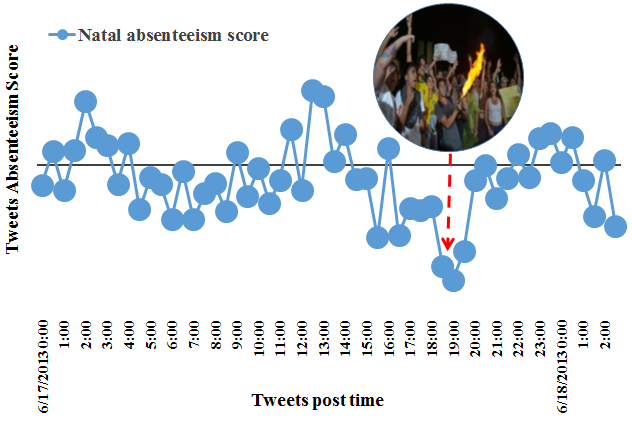
\includegraphics[width=3in]{figures/Natal_example1.png}
\caption{Detected group absenteeism in Natal, Brazil that began at 18:00 hours on June 17, 2013.
This absenteeism event coincides with a large protest that happened in the region.}
\label{fig:natal-protest}
\end{figure}


However, real-world activities are not always correlated with burst signals, and sometimes
are actually associated with unusually low level of activity occurred in social media. As shown in
Figure 1, in the city of
Natal, Brazil, a protest began at 17:00 hrs at the Museum of the Republic, with
people graduatlly joining the demonstration \footnote{http://www.jb.com.br/pais/noticias/2013/06/17/manifestantes-invadem-cobertura-do-congresso-nacional-em-brasilia/}. At the same time, on
Twitter, there was a {\it group absenteeism} behavior from 18:00 to 20:00 hrs on the
same day. As another example, Dec 24, 2013 experienced a
spate of floods in south Brazil. According to the Associated Press, more than 50,000 people have been forced to flee their homes in Minas Gerais and Espirito Santo states. Immediately following the occurrence of
the flood, Twitter activity in this region dropped by 51\%, and reached the lowest point on Dec 24, 2013. Some other examples include bus strikes in Brazil on May 21, 2014, an
earthquake in Chile on Apr 1st, 2014, and power supply disruption in Argentina on Dec 30, 2013
(see Table 2 in Section 4).

Investigating the phenomenon of unusually silent behavior of online users thus
holds enormous potential in understanding local societal events.
This paper presents the first study to systematically investigate the group absenteeism problem, and aims to answer the following three questions:
\begin{itemize}
\item How do we differentiate absenteeism from noise signals?
\item How do we efficiently identify absenteeism groups?
\item How do we gain insight into event detection based on our modeling of group absenteeism?
\end{itemize}

To answer these questions, we first consider the use
of Z-scores to measure the level of standard derivations of a time
series
(e.g., count of Tweets posted)
from its historical average for a given data object
in a given time interval. A lower Z-score is considered as a decreased level of activity. The
measure of absenteeism of a group (subset) of data objects is then defined in terms
of an aggregation function (e.g., summation) of Z-scores of data objects in this group, named as a
group-level Z-score. Secondly, an exhaustive search to identify groups with the lowest group-level Z-score is clearly impractical since there are $2^N$ candidate groups, where $N$ is the total number of data objects. Two different scenarios are considered. In the first scenario, data objects are embedded in a geographic domain and indexed by spatial coordinates. We propose an approach that relaxes convex hulls into rectangles to efficiently identify spatially connected areas as absenteeism groups. In the second scenario, data objects are embedded in a general graph as vertices. We propose an approach that efficiently identifies minimum weighted sub-graphs under sub-graph diameter constraints. To answer the third question, we conduct extensive experiments and discover evidence of significant relationships between the identified absenteeism groups in Twitter and real-world events collected from local news reports (e.g., natural disasters, protests).

\subsection*{Contributions.}
In answering the above research questions, we make several contributions. First, we study the phenomenon of group absenteeism using real Twitter datasets, and discuss useful score functions to measure the degree of absenteeism of a given group of data objects. Second, we formalize the group absenteeism detection problem as a subset minimization problem, and present two efficient approximation algorithms to detect the most absenteeism groups in two different scenarios, respectively: rectangle region search and minimal weight subgraph discovery. Finally, we conduct extensive experiments to analyze the strengths and weakness of these two algorithms and demonstrate their application to studying Twitter datasets over Latin America.

\iffalse
The rest of the paper is organized as follows. Section~\ref{sec:related} reviews related work and existing methodologies. Section~\ref{sec:algorithm} formalizes the group absenteeism problem, presents useful score functions, and designs efficient approximation algorithms. Section~\ref{sec:experiemnt} presents extensive experiments and comparisons, and Section ~\ref{sec:conclusion} suggests directions for future work.
\fi


%\begin{figure}[t]
%	\centering
%	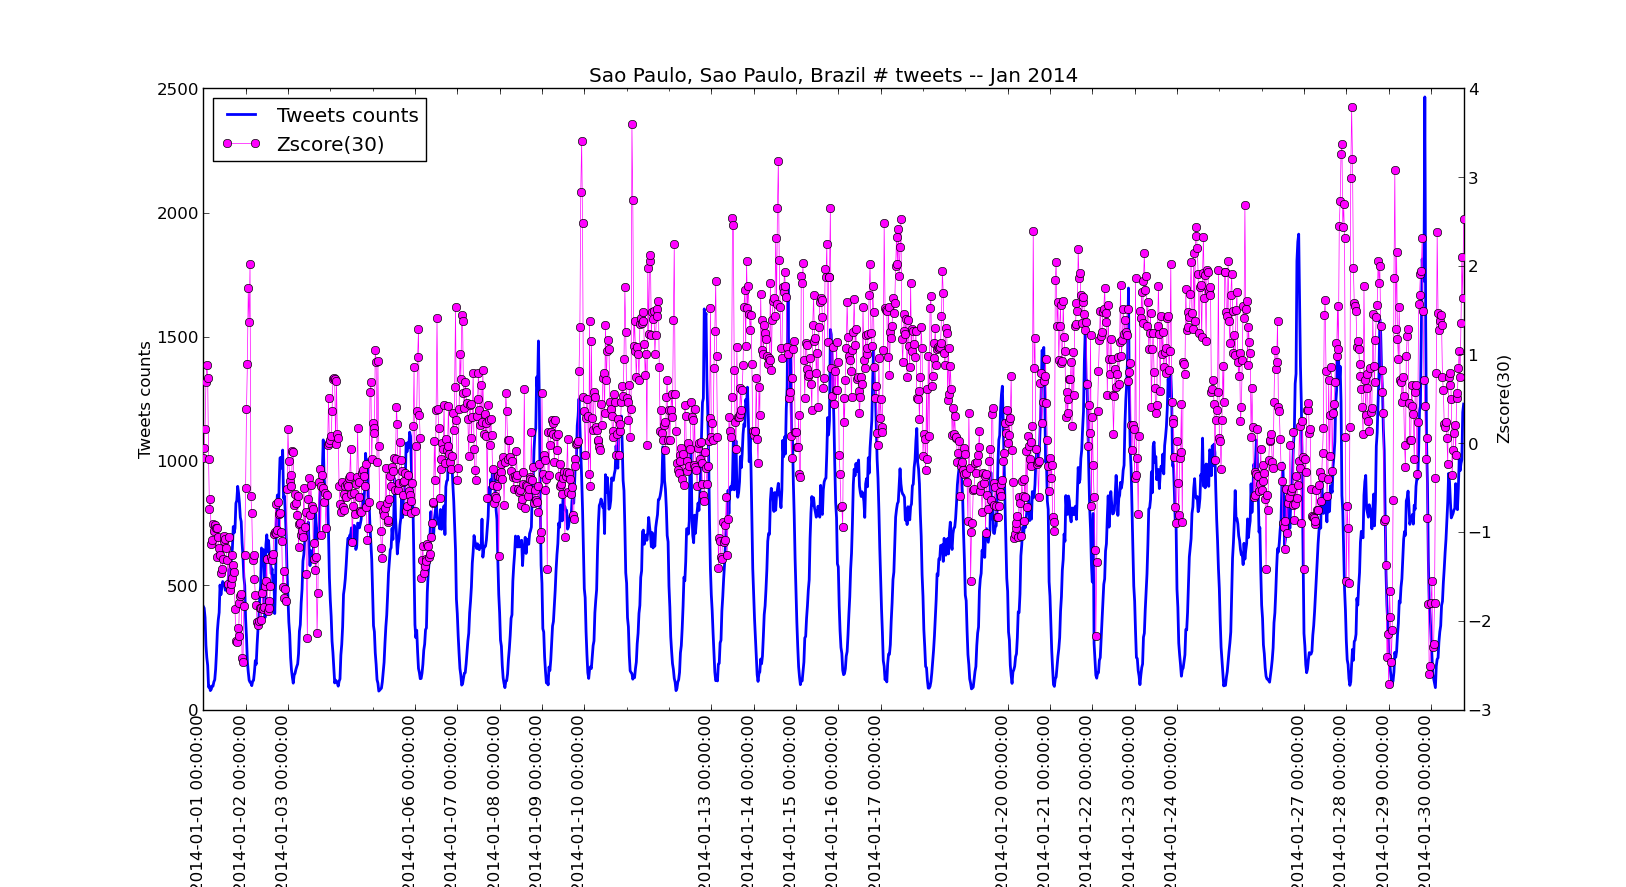
\includegraphics[width=3.3in, height=1.6in]{figures/tweets-period.png}
%	\caption{Tweets volume of January 2014 of Sao Paulo, Brazil. Blue curve shows tweets volume, and purple curve shows tweets zscore.
%	}
%	\label{fig:Tweets_volume}
%\end{figure}
%
%
%From Figure~\ref{fig:Tweets_volume}, we can see the Twitter activity has obvious periodicity of rises and falls pattern. Generally speaking, weekday has higher volume than weekends, and after midnight tweets tends inactive until the next day working time. To differentiate absenteeism signals from noise signals, we consider Z-score to measure for one time interval, how many standard derivations from its historical average for a given data object (e.g., count of tweets posted in a specific city).
%A $Z-score$ is defined by:
%\begin{equation}
%	\label{eq:zscore}
%	\begin{array}{l}
%		Z-score_t(n) =(X-\mathcal{M})/{\Sigma}\,
%	\end{array}
%\end{equation}
%where $X$ is the Twitter volume at time interval $t$, $\mathcal{M}$ is the trailing $n$-day moving average of the Twitter volume at time $t$, and $\Sigma$ is the standard deviation of those trailing $n$-day moving Twitter volume at time $t$. A lower Z-score is considered as the decreased level of activity of this data object. The measure of absenteeism of a group (subset) of data objects is defined as an aggregation function (e.g., summation) of Z-scores of data objects in this group, named as group-level Z-score. The detection of group absenteeism can be formulated as the identification of groups that have minimum group-level Z-score.
%

%
\section{Related work} \label{sec:related}
%\section{Related Work}
\paragraph{Burst event detection:}
Lappas et al.~\cite{lappas2009burstiness} define the temporal burstiness of a term using
the term frequency within one time interval, divided by the whole test period, and then 
minus the average term frequency. The authors further generalized their approach to detecting spatiotemporal bursts of certain terms in geocoded document streams~\cite{lappas2012spatiotemporal}. They use axis-oriented rectangles to constrain the selected regions to be spatially connected. Garcia-Gasulla et al.~\cite{garcia2014detection} discovered events based on collaborative social network data. Sakaki at al.~\cite{sakaki2010earthquake} considered Twitter users as social sensors to detect earthquakes. Rozenshtein et al.~\cite{rozenshtein2014event} detect events by capturing the compactness of a graph.

\paragraph{Spatial clustering:}
Spatial clustering groups the objects in a spatial data set and identifies contiguous regions in the space of the spatial attributes. Ng and Han~\cite{ng1994cient} proposed a clustering method called CLARANS based on randomized search that does not explicitly handle noise and requires users to predefine the number 
of clusters. Ester et al.~\cite{ester1996density} developed the density-based DBSCAN method
that is able to detect free shape clusters and does not require users to define the number of clusters. Cao et al.~\cite{cao2013analyzing} propose a supervised approach by using interestingness functions which assess the quality of spatial clusters based on uniformity measures to capture a domain expert's notion of uniformity. Recently, Rodriguez and Laio~\cite{rodriguez2014clustering} proposed a fast search clustering method to identify density peaks, which can remove outliers at the same time and does not require any predefined parameters.

\paragraph{Graph partitioning:}
The problem of graph partitioning consists of dividing the vertices in $g$ groups of predefined size, such that the number of edges lying between the groups is minimal~\cite{fortunato2010community}. The most popular algorithm is built around the idea of using centrality indices to find community boundaries~\cite{girvan2002community}. 
\iffalse
This algorithm is an iterative process with three components in each iteration: 1. Computation of the centrality for all edges;
2. Removal of edge with largest centrality: in case of ties with other edges, one of them is picked at random;
3. Recalculation of centralities for all the edges.
\fi
Karypis et al. developed a set of algorithms for partitioning graphs based on the the proposed multilevel recursive-bisection, multilevel k-way, and multi-constraint partitioning schemes~\cite{karypis2003multi, abou2006multilevel, lasalle2013multi}.

\noindent
As stated earlier our goal, distinct from burstiness detection, is to
design efficient algorithms for maximizing absenteeism score functions over possible groups.
Two different scenarios are considered. When data objects have geographic coordinates, we consider spatial clustering techniques to enforce spatial coherence of data objects in a possible absenteeism group. When data objects are organized as vertices in a general graph, we apply graph partitioning techniques to enforce graph coherence of data objects in a possible absenteeism group.

%
\section{Problem formulation} \label{sec:problem}
\subsection{Notations}
For ease of presentation, we first define the following notation:
\begin{itemize}
\item $c_i$ denotes city $i$, or we sometimes
use $c$ to mean a generic city without specifying the subscript $i$. $\mathcal{T}$ denotes
a set of cities, which is expressed as $\mathcal{T}=\{c_i\}$. $N=|\mathcal{T}|$ denotes
the number of cities in $\mathcal{T}$. In this paper, without specification, $\mathcal{T}$ denotes
all the cities in South and Central America.
\item $P$ is a subset of $\mathcal{T}$, and can be denoted as $P\in 2^{\mathcal{T}}$.
\item $d(c_i,c_j)$ denotes the distance of node $c_i$ and $c_j$, and is normalized w.r.t. the maximal distance in $\mathcal{T}$.
\item $d(P)$ is the maximal distance in $P$, which is also the diameter of $P$.
\item $\alpha(c)$ denotes city $c$'s Twitter absenteeism score expressed in terms
of Z-scores.
Using a geocoded Twitter collection as a dataset, based on every day's Tweets volume,
we calculate each city's Z-score. A Z-score is defined as:
\begin{equation}
	\label{eq:zscore}
	\begin{array}{l}
		\alpha(c)=Zscore_t(n) =(X-\mu)/{\sigma}\,
	\end{array}
\end{equation}
where $X$ is the tweet volume at time interval $t$, $\mu$ is the trailing $n$-day moving average of the
tweet volume at time $t$, and $\sigma$ is the standard deviation of those trailing $n$-day moving Tweets volume at time $t$. We typically
use $Zscore(30)$ as a figure of merit.

\item $A$ is the area threshold, and is normalized by the whole area of South and Central America.
\item $d_{th}$ is the distance threshold.
\end{itemize}


\subsection{Miller cylindrical coordinate system.}
We converted the 3-dimensional spherical coordinate into a 2 dimensional
set of coordinates using the Miller cylindrical projection algorithms. %The conversion error is negligible because in most case the the size of $P_{min}$ is relatively small.
Since we are only interested in cities of Latin America, we set the center point of Latin
America as the original point in the Miller cylindrical coordinate system. Suppose that $c$'s latitude and longitude are $lat$ and $lon$; then $c$'s location in the Miller coordinate conversion can be written as:
\begin{equation}
x = lon - lon_0
\end{equation}
\vspace{-5mm}
\begin{equation}
y = 1.25*ln[tan(\frac{1}{4}\pi+\frac{2}{5}(lat-lat_0))],
\end{equation}
where $(lat_0,lon_0)$ is the center point of South American.
%Figure~\ref{fig:Brazil_regional_June20} plots the cities in the Miller cylindrical coordinate system.
In the rest of
this paper, all city locations refer to positions in the Miller cylindrical coordinate system.
\begin{figure}[t]
	\centering
	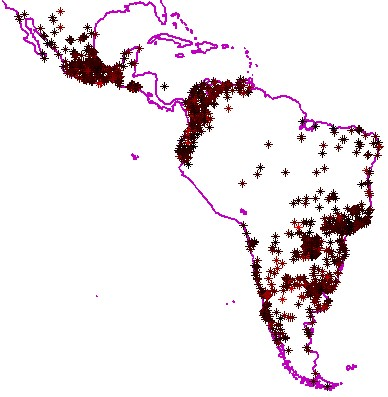
\includegraphics[width=1.5in]{figures/zscore.png}
	\caption{Absenteeism scores of 1290 cities in South American on May 16, 2014. One `*' point represents one city, and the darker the color is, the lower the its absenteeism score.}
	\label{fig:city_south_american}
\end{figure}


\subsection{Problem formulation}
 Figure~\ref{fig:city_south_american} plots the 1290 cities in Latin America
on May 16, 2014. Each city's absenteeism score is presented by its color. The darker the color is, the lower the city's absenteeism score is. We are interested with a city group, $P_{min}$ with the lowest absenteeism score. Usually, we require that all the cities in $P_{min}$ are close to each other. In this paper,  $P_{min}$ is required to meet one of the two constraints.

\paragraph{regional constraint} $P_{min}$ can be covered by
a convex polygon with areas less than $A$. With this constraint, we use $\Gamma_1(P)$ to denote $P$'s group absenteeism score, which can be expressed as:
 \begin{equation}
\Gamma_1(P)=\sum_{c_i\in H(P)} {\alpha(c_i)}
\end{equation}
The problem can be expressed as:

 \begin{equation}
 P_{min}=\argmin\limits_{P\in 2^\mathcal{T}, s(P)\leq A}\Gamma_1(P)
\end{equation}

 \paragraph{subgraph constraint}For any two cities in $P_{min}$, the distance between them is less than $d_{th}$. In this constraint, we use $\Gamma_2(P)$ to denote $P$'s group absenteeism score, which can be expressed as:
 \begin{equation}
\Gamma_2(P)=\sum_{c_i\in P} {\alpha(c_i)}
\end{equation}
The goal then is:
 \begin{equation}
 P_{min}=\argmin\limits_{P\in 2^\mathcal{T}, s(P)\leq A}\Gamma_2(P)
\end{equation}



\section{Absenteeism group detection algorithms} \label{sec:algorithm}
%\section{Absenteeism group detection algorithms}
The optimal solution to the problem in last section has running time complexity of $O(2^N)$. To reduce the time complexity, in this  section, we propose two approximate optimal solutions, the first is regional approach with time complexity of $O(N^3)$, and the second is subgraph approach, with $O(N^2)$ time complexity.
\subsection{Regional approach}
For further explanation convenience, we define some notations firstly.
\begin{itemize}
  \item Suppose $H(P)=P$, $P$ is called an empty convex polygon, which means all the nodes in $P$ lie in the edges of $H(P)$, and there is no node lies inside of $H(P)$. $P$ is empty does not necessary mean that there is no any city in $\mathcal{T}$ happen to lie inside the convex polygon of $P$, it just mean that $P$ does not contain any node which lies inside $H(P)$. As shown in Figure~\ref{fig:notation}, $P_1=\{c_1,c_2,c_3,c_4\}$ and $P_2=\{c_5, c_6, c_7, c_8, c_9\}$. $P_1$ is empty because $H(P_1)=P_1$. While $P_2$ is not an empty convex polygon, since $H(P_2)=\{c_5, c_6, c_7, c_8\}\neq P_2$.
    \item Suppose $P$ is an empty convex polygon, $g(P)$ is used to represent cities which either lie in the edges of $P$, or inside $H(P)$. We call $g(P)$ is $P$'s domain, and $P$ is the support of $g(P)$. As shown in Figure~\ref{fig:notation}, $P_1$ is an empty convex polygon, and inside $P_1$, there are nodes $c_{11}, c_{12}$, thus $g(P_1)=\{c_1,c_2,c_3,c_4,c_{11},c_{12}\}$.
\end{itemize}

\begin{figure}[t]
	\centering
	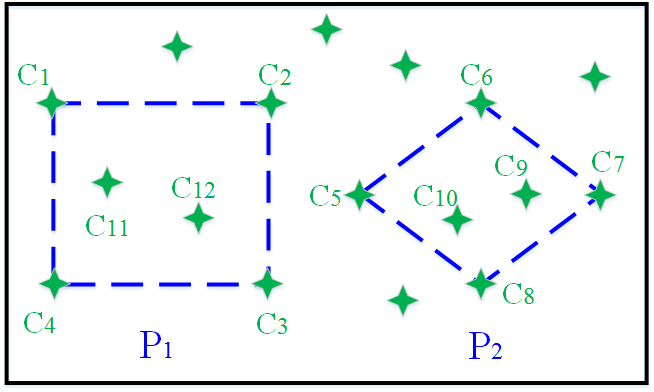
\includegraphics[width=2.2in,height=1.3in]{figures/bruteforce.png}
	\caption{Notation explanation: $P_1=\{c_1,c_2,c_3,c_4\}$, $P_2=\{c_5, c_6, c_7, c_8, c_9\}$. $P_1$ is empty convex polygon, while $P_2$ is not because $H(P_1)=P_1$, and $H(P_2)=\{c_5, c_6, c_7, c_8\}\neq P_2$. $P_1$ is an empty convex polygon, which does not mean there is no any node in $P_1$. Instead, inside $P_1$, there are nodes $c_{11}, c_{12}$, thus $g(P_1)=\{c_1,c_2,c_3,c_4,c_{11},c_{12}\}$.}
	\label{fig:notation}
\end{figure}


\subsubsection{Brute force algorithm}
An obvious brute force algorithm for minimal absenteeism group detection is described in algorithm~\ref{algo:convex_hull}.
\begin{enumerate}
  \item Firstly, it finds out all the empty convex polygons, $\mathcal{P}= \{P_i\}$, $s(P_i)\leq A$, $\forall P_i\in 2^\mathcal{T}$;
  \item Secondly, for each $P_i \in \mathcal{P}$, compute $P_i$'s domain $g(P_i)$, and its group absenteeism score $\Gamma_1(P_i)$;
  \item return the minimal $\Gamma_1(P_i)$, and the corresponding empty convex polygon $P_i$.
\end{enumerate}

\begin{algorithm}[h]
\centering
\captionsetup{font=scriptsize}
\caption{Brute force algorithm}
{\footnotesize \begin{algorithmic}[1]
\STATE {\bf Input:} city set $\mathcal{T}$, score set $\alpha(\mathcal{T})$ and areas upper bound $A$
%, \alpha(\mathcall{T})$: set of sources for location $l$; ${\bf D_l}$: training points; $R_{S_l}$: source-topic relevance dictionary for sources in $S_l$ and points in ${\bf D_l}$; $O_{S_l}$: one-class SVMs for $S_l$; $\epsilon$: discount factor
\STATE {\bf Output:} subset $P$ with lowest absenteeism score, where $P\in 2^{\mathcal{T}}$	
	\FORALL {$K$ from 3 to $N$}
			\FORALL {$P_i$}
			\STATE{enumerate all city set $P_i$, where $|P_i|=K$}
			\IF {$P_i$ is empty}			
					\IF {$s(P_i)\leq A$}
						\STATE{compute $P_i$'s domain $g(P_i)$}
						\STATE{compute group absenteeism score $\Gamma_1(P_i)$}
					\ENDIF
			\ENDIF
	\ENDFOR	
	\ENDFOR	
\RETURN $\min\Gamma(g(P_i))$, and $P_i$
\end{algorithmic}}
\label{algo:convex_hull}
\end{algorithm}


The purpose of introducing the concept of empty convex polygon is to avoid unnecessary duplicated computation. As shown in figure~\ref{fig:notation}, for city sets $Q_1=\{c_5, c_6, c_7, c_8\}$, $Q_2=\{c_5, c_6,c_7, c_8, c_9\}$, $Q_3=\{c_5, c_6, c_7, c_8, c_{10}\}$, and $Q_4=\{c_5, c_6,c_7, c_8, c_9, c_{10}\}$, we can see that $H(Q_1)=H(Q_2)=H(Q_3)=H(Q_4)$. If we do not differentiate those city sets by introducing empty convex polygon, the group absenteeism for set $\{c_5, c_6, c_7, c_8, c_9, c_{10}\}$ would be computed four times. However, with the concept of empty convex polygon, only $Q_1$ will be chosen to compute the group absenteeism scores, and all the other three city sets will be discarded directly.

The basic idea of brute force algorithm is to enumerate all the possible convex polygon in $\mathcal{T}$. For the worst case, there are $O(2^N)$ convex polygons, which makes the brute brute-force algorithm impractical to realize. When $|P_i|=K$, the above algorithm need to enumerate all the $C_N^K$ cases. For each case, we use the classical $GRAHAM-SCAN$ algorithm, which has $O(KlogK)$ running time complexity to decide whether $P_i$ is empty or not. To compute $P_i$'s domain $g(P_i)$ and $\Gamma_1(P_i)$, it's complexity is $O(N)$.
Thus, when $|P_i|=K$, the complexity could be expressed as: $t(K)=K*logK*N*C_N^K$, therefore the overall complexity could be expressed as:
\begin{equation} \label{e1.1}
T=\sum_{n=3}^Nn*logn*N*C_N^n\ge O(N2^N)
\end{equation}
%$$T=\sum_{K=3}^Nt(K)=\sum_{K=3}^NK*logK*N*C_N^K\ge N*2^N.$$
From the analysis above, we can see that the complexity of convex hull minimal absenteeism group detection is too complicated considering that $N$ is usually more that 1000.

\subsubsection{Rectangle approximate algorithm}

For explanation convenience, we define some notes firstly.
\begin{itemize}
  \item $\mathcal{R}(c_i,c_j)$ means a rectangle areas, which is defined by node $c_i$ and $c_j$, where $c_i$ is the most left-top node, and $c_j$ is the most right-bottom node. $\mathcal{R}(c_i,c_j)$ also denotes the all nodes which lies in that rectangle area. Sometimes, we also use $\mathcal{R}$ without specifying $c_i$ and $c_j$.
    \item $s(\mathcal{R})$ means the areas of rectangle $\mathcal{R}$.
    \item Suppose $s(\mathcal{R})\leq A$, $\mathcal{R}$ is called a qualified rectangle.
\end{itemize}

\begin{figure}[t]
	\centering
	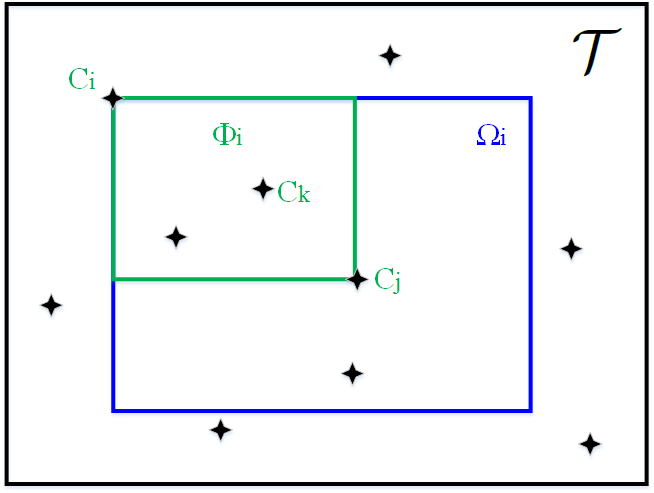
\includegraphics[width=2in,height=1.3in]{figures/algorithm.png}
	\caption{Rectangle region search algorithms.}
	\label{fig:rectangle_region}
\end{figure}

From the above analysis, we can see that the convex hull detection algorithm is too complex to realize. The root of this complexity lies in that we need to enumerate all the subset of $2^{\mathcal{T}}$.
To simplify our problem, we assume that the absenteeism region is a rectangle. Hence, the problem is transformed as: Given city set $\mathcal{T}$, areas upper bound $A$, determine the rectangle area
 \begin{equation}
 \mathcal{R}_{min}=\argmin\limits_{R\in 2^\mathcal{T}, s(\mathcal{R})\leq A}\Gamma_1(\mathcal{R})
\end{equation}

The rectangle minimal absenteeism group detection algorithm is described in Algorithm~\ref{algo:rectangle}.

\begin{algorithm}[t]
	\centering
	\captionsetup{font=scriptsize}
	\caption{Rectangle approximate algorithm.}
	{\footnotesize \begin{algorithmic}[1]
			\STATE {\bf Input:} city set $\mathcal{T}$, score set $\alpha(\mathcal{T})$ and areas upper bound $A$.
			\STATE {\bf Output:} rectangle $\mathcal{R}_{min}$ with lowest absenteeism score.
			\FORALL {each $c_i\in \mathcal{T}$}
			\STATE {assume $c_i$ as the most left-top point}	
			\STATE {select set $\Omega_i=\{c_j\}$; $\forall c_j\in \Omega_i, s(\mathcal{R}(c_i,c_j))\leq A$}
			\FORALL {each $c_j\in \Omega_i$}
			\STATE {compute group absenteeism score $\Gamma(\mathcal{R}(c_i, c_j))$}
			\ENDFOR	
			\STATE compute $\Gamma_{c_i}=\argmin\Gamma(\mathcal{R}(c_i, c_j))$, 	$\forall c_j\in \Omega_i$
			\ENDFOR
			\STATE{compute the $\Gamma_{min}=\argmin\Gamma_{c_i}, \forall c_i\in \mathcal{T}$}
			\RETURN $\Gamma_{min}$ and  $\mathcal{R}_{min}$.
		\end{algorithmic}}
		\label{algo:rectangle}
	\end{algorithm}
	
	
	
\begin{enumerate}
  \item Firstly, for each node $c_i\in \mathcal{T}$, it finds out the node set $\Omega_i$, such that $\forall c_j \in \Omega_i, \mathcal{R}(c_i, c_j)\leq A$. This step means when we fix $c_i$ as the most left-top vertex, then identify all the qualified rectangles. This step time complexity is $O(N)$.
\item Secondly, for each node $c_j \in \Omega_i$, compute group absenteeism score $\Gamma(\mathcal{R}(c_i,c_j))$, and then compute the $\Gamma_{c_i}=min\Gamma(\mathcal{R}(c_i, c_j))$ for all $c_j\in \Omega_i$. This step's time complexity depends on the node numbers of $\Omega_i$, which is denoted as $|\Omega_i|$. Suppose that nodes are uniformly distributed, thus $|\Omega_i|$ is directly proportional to $A$. Thus, this step's time complexity can be expressed as A, which is constant.
  \item Lastly, it returns the minimal $\Gamma_{min}=\Gamma_{c_i}, \forall c_i\in \mathcal{T}$.
\end{enumerate}
From the analysis, the rectangle algorithm time complexity is $A*N*A*N*N = O(N^3)$, which is greatly reduced comparing with the brute force algorithm.
%Figure~\ref{fig:mCoornidate} shows the most rectangle absenteeism group on Sep 11, 2013, when we set $A=0.02$.




\subsection{Subgraph approach}
For explanation convenience, we define some mathematic notation firstly.
\begin{itemize}
 \item $\mathcal{T}^-$ represents cities in $\mathcal{T}$ with negative absenteeism score, and can be expressed as $\mathcal{T}^-=\{c_i\}; \forall c_i\in \mathcal{T}$ and $\alpha(c_i)< 0$.
    \item Given city $c_i$ and distance threshold $d_{th}$, $\xi(c_i)$ means the cities whose distance to $c_i$ is closer than $d_{th}$. $\xi(c_i)$ can be expressed as $\xi(c_i)=\{c_j\}; \forall c_j\in \mathcal{T}$ and $d(c_i,c_j)< d_{th}$.
\end{itemize}
Essentially, a city set $\mathcal{T}$ is equivalent with an complete graph $G$, and any two cities $c_i$, and $c_j$ in $G$ are connected with distance of $d(c_i,c_j)$. The city absenteeism scores are mixed by both positive and negative ones. However for most circumstances, we are only interested with the cities which have the negative absenteeism scores, and are physically close enough to each other. Thus, we can think city set $\mathcal{T}^-$ into an complete graph, and identify the optimal subgraph $P_{min}$ which has the minimal group score, while its diameter $d(P_{min})\leq d_{th}$.\\
Thus, the problem is transformed as: Given city set $\mathcal{T}^-$, distance threshold $d_{th}$, identify city set $P_{min}\in 2^\mathcal{T^-}$, such that

 \begin{equation}
 P_{min}=\argmin\limits_{P\in 2^\mathcal{T^-}, s(P)\leq A}\Gamma_2(P)
\end{equation}

\begin{algorithm}[h]
	\centering
	\captionsetup{font=scriptsize}
	\caption{Subgraph approximate algorithm.}
	{\footnotesize \begin{algorithmic}[1]
			\STATE {\bf Input:} city set $\mathcal{T}$, score set $\alpha(\mathcal{T})$ and $d_{th}$.
			\STATE {\bf Output:} Subgraph $P_{min}$ with lowest absenteeism score
			\STATE find out $\mathcal{T}^-$ and $\alpha(\mathcal{T}^-)$
			\FORALL {$c_i \in \mathcal{T^-}$}
			\STATE identify $c_i$'s neighbors $\xi(c_i)$
			\STATE compute $\Gamma(\xi(c_i))$ 	
			\ENDFOR
			\RETURN ${P_{min}}$  and $\xi(c_i)$
		\end{algorithmic}}
		\label{algo:Subgraph}
	\end{algorithm}
	

\begin{table*}[t] %!htp
	\renewcommand{\arraystretch}{1}
	\caption{\label{table:list_events} Detected absenteeism groups over all the South America countries}
	\scriptsize
	\centering
	%\begin{tabular}{ p{3.5cm} | p{3.2cm} |p{2.9cm} | p{2.9cm} | p{2.9cm}}
	\begin{tabular}{ p{0.4cm}|l|l| p{8cm}|l | l}
		\hline
		\textbf{No.} & \textbf{Date}& \textbf{Country}& \textbf{ Events} & \textbf{ Period}  &  \textbf{ Method}   \\ [1ex]
		\hline
        1& 2013-06-20 & Brazil & Brazilian Spring: Protests in over 100 cities, over 2 million people &one day& Subgraph, regional \\
        2& 2013-08-31 & Peru & Peru snow state of emergency extended to more regions & one day&regional \\
        3& 2013-09-03 & Venezuela & Power cut leaves much of Venezuela without electricity &one day& subgraph\\
		4& 2013-09-11 & Mexico & Mexico teachers protest against education reform in 17 cities &15:00-15:30 &Subgraph \\
        5& 2013-10-17 & Colombia & Floods, particularly heavy rains affecting south-west of Colombia & one day& regional \\
        6& 2013-12-24 & Brazil & Floods, more than 50,000 people are forced to flee their homes&one day& subgraph, regional \\
        7& 2013-12-30 & Argentina &  Power supply disrupted in heatwave in Buenos Aires, Argentina. &one day&subgraph\\
        8& 2014-01-09 & Bolivia & Floods & one day&regional, subgraph \\
        9& 2014-01-31 & Chile & Chile`S IPSA stock index hit lows not seen in over 4 years & one day&regional\\
        10& 2014-02-12 & Bolivia & Heavy rain caused floods and landslides in several parts of Bolivia &one day& regional, subgraph\\
        11 & 2014-02-13 & Argentina & Heavy rain and landslides & one day&subgraph\\
        %12& 2014-02-19 & Venezuela & Earthquake M5.5, 49000 people exposed to strong shaking &6:30AM &regional \\
        12& 2014-02-27 & Venezuela & Social unrest & one day&subgraph, regional \\
        %14& 2014-03-15 & Peru& Earthquake shaking up to Very Strong for 45 000 people &17:30PM &subgraph \\
        13& 2014-03-24 & Chile & People in Chile on edge over unusual string of 300 tremors &one day&subgraph\\
        %16& 2014-03-31 & Chile & Earthquake M5.6 &7:30AM &subgraph\\
        14& 2014-04-01 & Chile &  M8.2 earthquake struck off the coast of Chile, epicenter is Iquique & 20:45-20:50 &subgraph \\
        15& 2014-05-01 &Central America& Labor Day, national holiday &one day &Subgraph, regional \\
        16& 2014-05-16 & Brazil & Anti-World Cup protests in 12 cities of Brazil &one day& subgraph, regional \\
        17& 2014-05-21 & Brazil & Bus strike paralyzes Brazil's biggest city as World Cup looms &9:30-10:00& regional\\				
		\hline
	\end{tabular}
\end{table*}



An obvious brute force algorithm would be enumerate all the possible $P\in 2^\mathcal{T^-}$, thus the complexity would be $2^{N^-}$. Usually $N^-$ is larger than 100, which makes the brute force algorithm uncritical. Algorithm~\ref{algo:Subgraph} gives out an approximate algorithm with $O(N^2)$ running time complexity.
\begin{enumerate}
  \item Firstly, it determines the subset $\mathcal{T}^-$ since we only concern the negative absenteeism cities.
  \item Secondly, for each node $c_j \in \mathcal{T}^-$, it identifies neighbor $\xi(c_i)$ and $\Gamma(\xi(c_i))$. In $\xi(c_i)$,  each node's distance to $c_i$ is smaller than $d_{th}$. $\forall c_{j1}, c_{j2}\in \xi(c_i$ and $c_{j2}$ , $d(c_{j1}, c_{j2})\leq d(c_{j1}, c_i)+d(c_{j2}, c_i)\leq 2d_{th}$. Thus, this approximate algorithm can guarantee the diameter of $P_{min}$ is less than $2d_{th}$. Evidently, this step's time complexity is linear because it need to enumerate $c_i$ to all other node in $\mathcal{T}^-$.
  \item Lastly, it returns the minimal $\Gamma_{min}=\Gamma_{c_i}, \forall c_i\in \mathcal{T}$.
\end{enumerate}




% % % % % % % % % % % % % the end % % % % % % % % % % % % %

%
\section{Experimental results} \label{sec:experiemnt}

\subsection{Experiment Setup}
\paragraph{Dataset:}
The study described in this paper uses datasets of South American Tweets, collected over 12 months (from May 2013 to May 2014), covering 22 countries. Our Twitter dataset was built from querying Datasift's streaming API. Tweets from GPS-enabled devices also report latitude/longitude coordinates. However the percentage of such Tweets in the collected sample was too low to be useful.

\paragraph{Geocoding:}
For this study, we build a geocoding tool to lookup each Tweet's location. To get a higher recall of geo-located Tweets, we apply our own geocoding library - that uses World Gazettee~\cite{worldgazetteer} database to lookup location names and geo-coordinates. For event geolocation we look into Tweet's text for string matches to location (cities, admin, country) and landmark place names such as Plaza de la Independencia (Quito, Ecuador). In cases, where no event location was found in Tweet's text, we use geo-coordinates or self-reported location string in Tweet's metadata.

Using above described pipeline, we were able to extract the geolocated $598,300$ cities from South American Twitter. Since many geolocated Tweets are really sparse within one day, we only consider the 1290 cities whose daily average Tweets larger than 100.

\paragraph{Major events labels:}
We focus on two kinds of major events, one is natural disasters, eg., earthquake, floods, and landslides, that we found from European Emergency Response Coordination Center(ERCC)~\footnote{http://erccportal.jrc.ec.europa.eu/} and World Top Stories Timeline~\footnote{http://www.mapreport.com/}; the second one is major social unrest events. We define major mass protest events by checking a gold standard report(GSR) in Latin America provided by MITRE.


\subsection{Group absenteeism detection results}
Using the geocoded Tweets as dataset, based on every day's Tweets volume, we calculate each city's Z-score. We set the time interval in two levels, a small-grained level (30 minutes), which is used to see if it connect with emergence events, the big-grained level is one day, which used to see if it associates with long-term events. When we set the time interval as half hour, then for half hour of that day, we calculate their respective Z-score(30) based on their previous 30 days' time slot Tweets count. For example, Jan 31, 2014's Z-score(30) at 8AM is got by previous 30 days Tweets counts at 8AM. If the time interval is one day, when calculate a weekday's Z-score(30), only use the previous 30 weekdays Tweets count to calculate. To calculate a weekend day's Z-score(30), only use previous 30 weekend days. The lowest absenteeism score means the most obvious absenteeism behavior. Set the test period from Jun 01, 2013 to May 31, 2014, for each day, employ the algorithms described above, and select the most absenteeism group of that day. For the one day time interval, each day will get one absenteeism group; for the 30 minutes time interval, will get 48 absenteeism groups for every half an hour, we pick the lowest group score.


After get a whole year absenteeism groups of each day, then we try to discover what events are going on of those absenteeism groups. How to decide whether an absenteeism group associate with major events? Of each absenteeism group, if there is one city coincide with the major events area, we take it as associated with the major events.
%Of the whole year absenteeism groups, not all the selected groups have major events, sometimes it is difficult to decide if they associate with major events.
Compared with the ERCC and GSR records, we list 17 groups which associate with major events, in Table~\ref{table:list_events}.

On Jun 20, 2013, set time interval as one day, for regional algorithm we set $A$ as 0.02, and for subgraph algorithm, we set $d_{th}$ as 0.1, we get two set of absenteeism groups which associate with Brazil spring events, plotted in Figure~\ref{fig:20130620}. With the same setting, we also plot the absenteeism groups on May 01, 2014, which shows the central America Labor Day's group absenteeism distribution, see Figure~\ref{fig:labor_day}.

On Sep 11, 2013, using subgraph algorithm, we found the absenteeism group at 15:00 is the lowest. By checking the GSR record, we find on Sept 11, 2013, there were 17 cites in Mexico having protests demonstration. Using the minimal weight graph algorithm, of the selected 20 absenteeism cities, 6 of them involved in the teachers' protest events. This shows huge protest events can result in high group absenteeism phenomenon.


\begin{figure}[t]
	\centering
	\subfigure[regional]{
		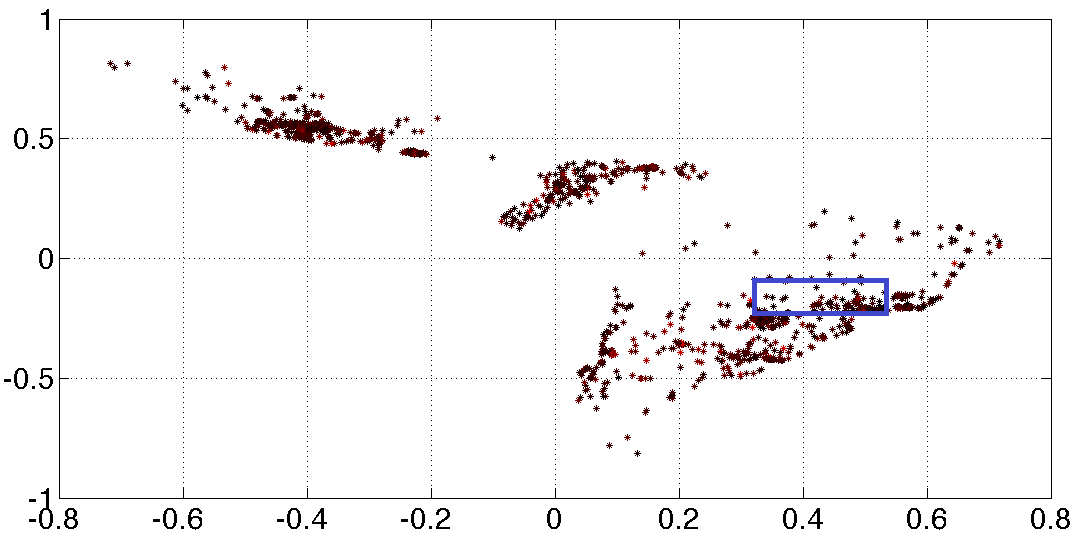
\includegraphics[width=1.55in,height=1.55in] {figures/Brazil_regional_20130620.png}
		\label{fig:Brazil_regional_June20}
	}
	\subfigure[subgraph]{
		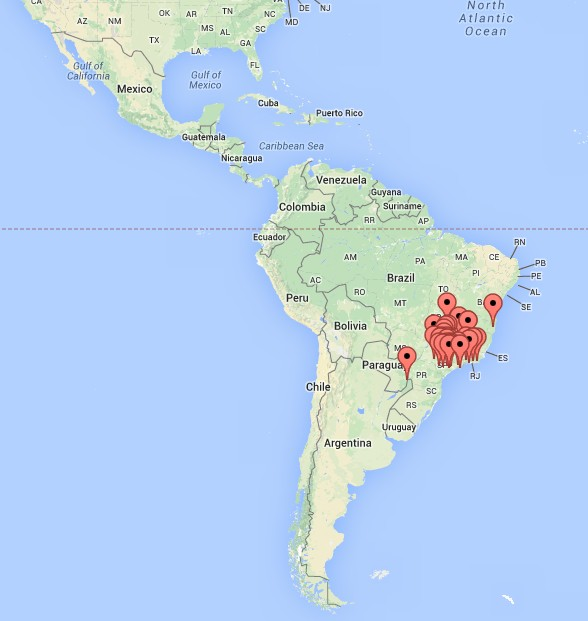
\includegraphics[width=1.55in,height=1.5in] {figures/Brazil_subgraph_20130620.jpg}
		\label{fig:Brazil_subgraph_June20}
	}
	\vspace{-1em}
	\caption{ The selected absenteeism group in South American on June 20, 2013.}
	\label{fig:20130620}
\end{figure}

\begin{figure}[t]	
	\centering
	\subfigure[regional]{
		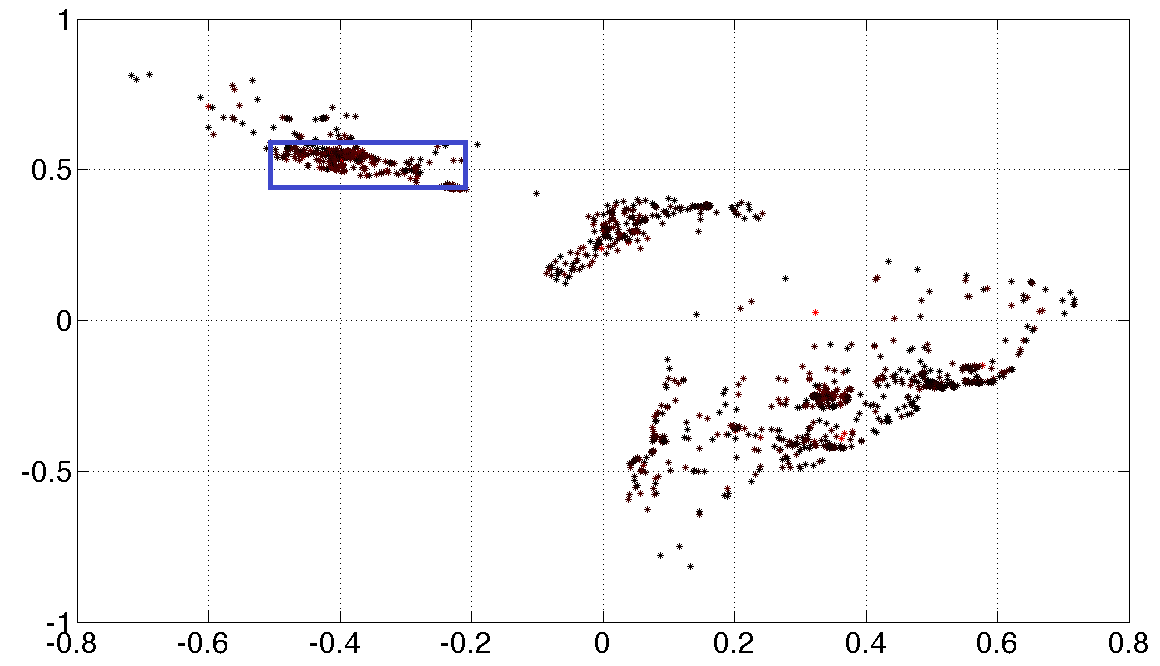
\includegraphics[width=1.55in,height=1.55in] {figures/regional_labor_day.png}
		\label{fig:Mexico_regional}
	}
	\subfigure[subgraph]{
		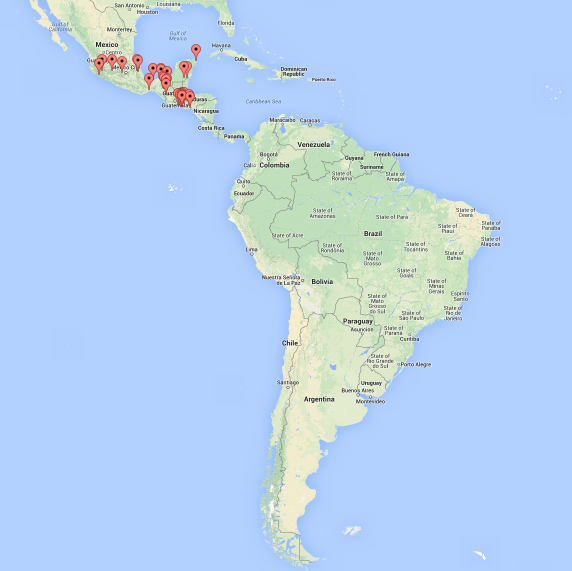
\includegraphics[width=1.55in,height=1.5in] {figures/subgraph_labor_day.png}
		\label{fig:Mexico_subgraph}
	}
	\vspace{-1em}
	\caption{ The selected absenteeism group in South American on May 1st, 2014.}
	\label{fig:labor_day}
\end{figure}


\subsection{Comparison of different algorithms}
We use the data set on February 27, 2014, and set the time window as one day. We plot the comparison results from two aspects:  running time complexity, and parameter sensibility in figure~\ref{fig:performance},~\ref{fig:running_time},~\ref{fig:sensibility}.
\begin{figure}[h]
	\centering
	\subfigure[regional]{
		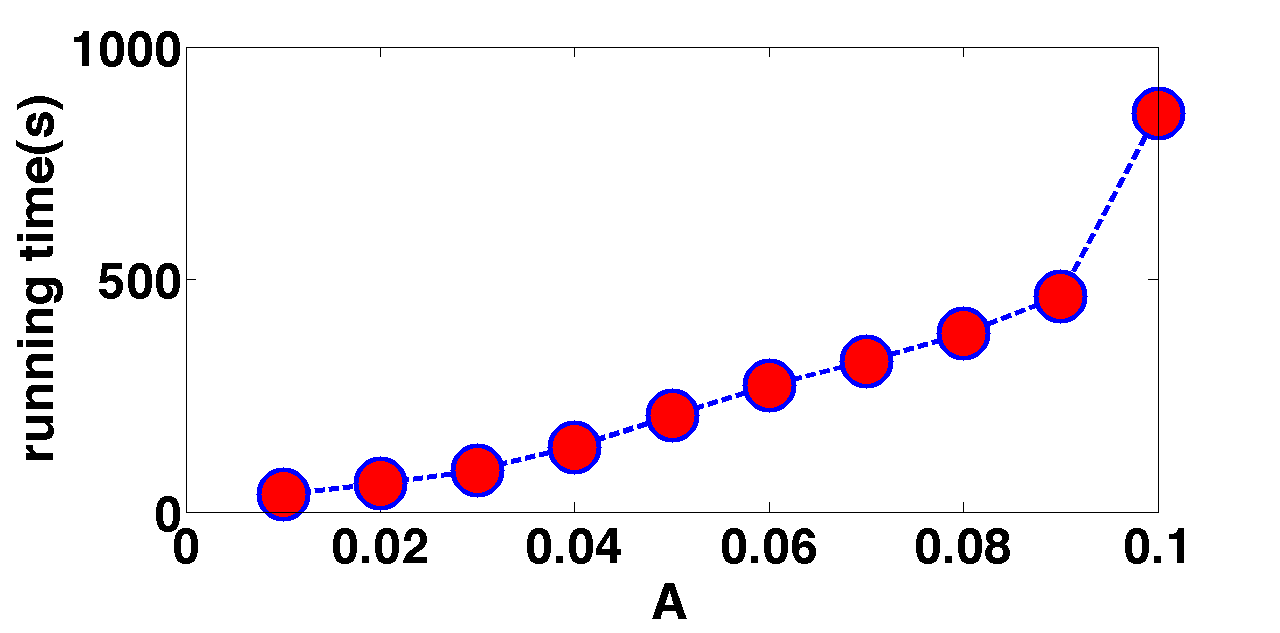
\includegraphics[width=1.55in,height=1in] {figures/performance1.png}
		\label{fig:performance1}
	}
	\subfigure[ubgraph]{
		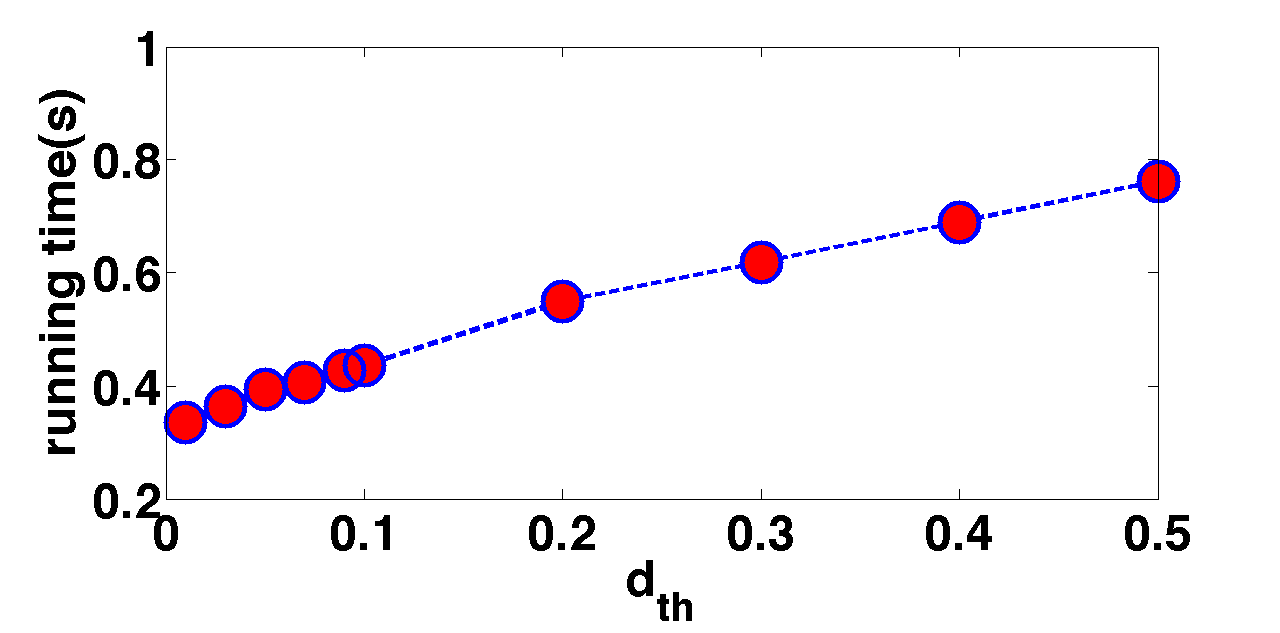
\includegraphics[width=1.55in,height=1in] {figures/performance2.png}
		\label{fig:performance2}
	}
	\vspace{-1em}
	\caption{running time vs input parameter.}
	\label{fig:performance}
\end{figure}
\paragraph{Running time}From Figure~\ref{fig:performance}, we can see that the running time of regional approach increases extremely fast when $A$ is larger than 0.09. While in subgraph approach, the increasing speed is much stable as $d_{th}$ increases. This is because regional approach's time complexity is in proportion to $A^2$, while subgraph approach's time complexity is proportional to $d_{th}$. From Figure~\ref{fig:running_time}, we can see clearly that for the regional algorithm, the running time complexity also increase sharply with the input size $n$, while in subgraph approach, the increase speed is moderate. This is because the regional approach's timing complexity is $O(N^3)$, while subgraph approach's time complexity is $O(N^2)$. Thus, the subgraph approach is better  than regional approach in term of running time for a larger absenteeism group.
\begin{figure}[h]
	\centering
	\subfigure[regional]{
		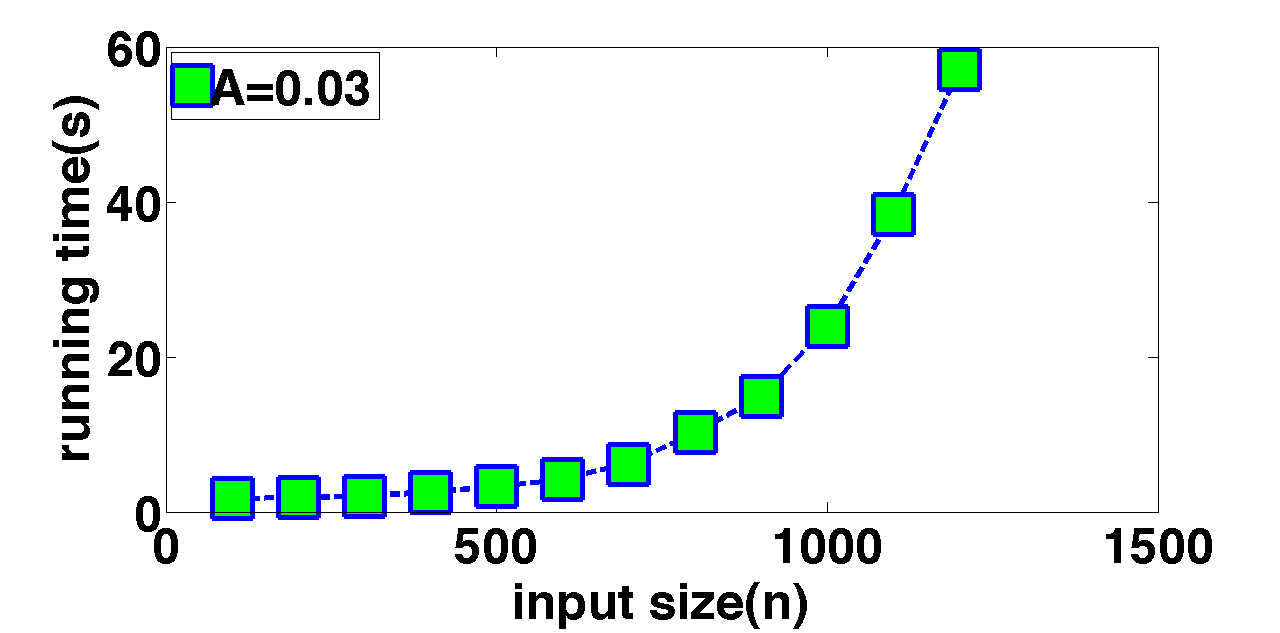
\includegraphics[width=1.55in,height=1in] {figures/running_time1.png}
		\label{fig:running1}
	}
	\subfigure[subgraph]{
		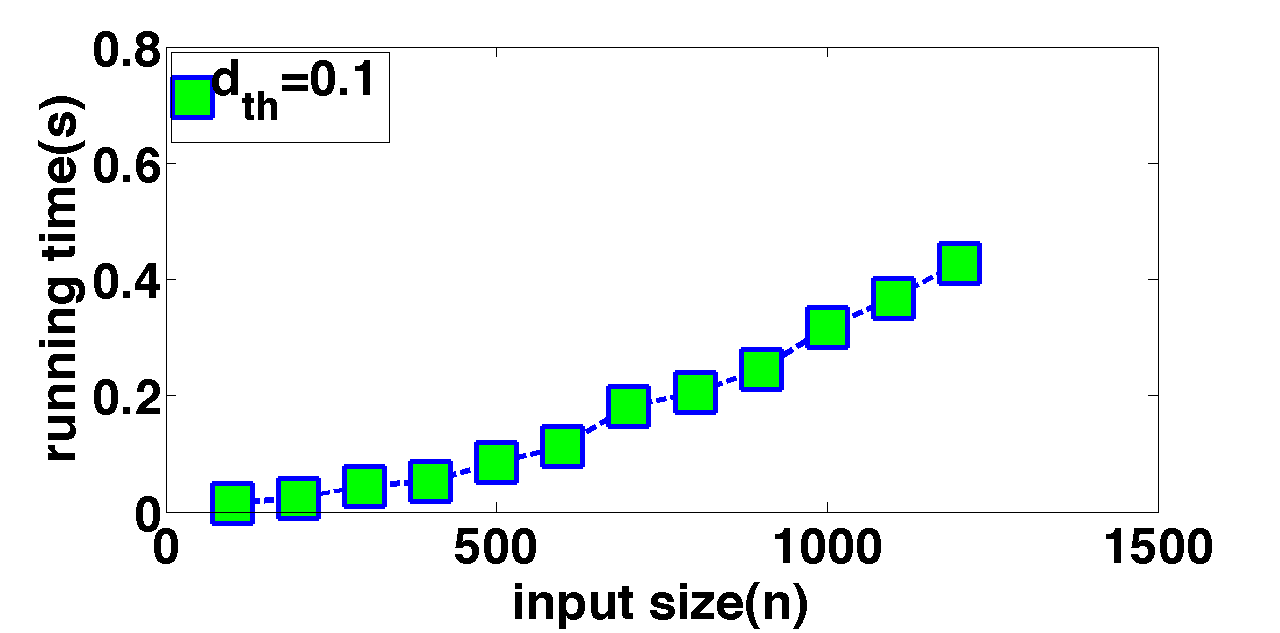
\includegraphics[width=1.55in,height=1in] {figures/running_time2.png}
		\label{fig:running2}
	}
	\vspace{-1em}
	\caption{Running time vs input size.}
	\label{fig:running_time}
\end{figure}
\paragraph{Parameter sensibility}In regional approach, set the input parameter as $A$, and the optimal absenteeism group as $P_{min}$. When $A$ is changed to $A$', the optimal absenteeism group is changed to $P_{min}$, define the output error as the city number that exists in $P_{min}$ but not in $P_{min}'$, and denoted as $P_{min}-P_{min}'$. We define the parameter sensibility as: $$sensibility=\frac{{|P_{min}-P_{min}'|}/{|P_{min}|}}{|A-A'|/{A}}.$$ We plot the regional approach and subgraph approach's sensibility in Figure~\ref{fig:sensibility}. In the regional approach, when the input parameter error is smaller than 20\%, the output absenteeism group error is less than 5\%. While in the subgraph approach, the output absenteeism group error is linear to the input error parameter. This is probably because regional approach aggregates all the absenteeism score covered by the region, and usually has a much larger city number than the subgraph approach, and makes regional approach better at anti-noise.  All in all, the regional algorithm focuses on all the cities in the cover group, and has a better global performance at anti-noise, while is inferior to the subgraph counterpart in term of running time complexity.
\begin{figure}[h]
	\centering
	\subfigure[regional]{
		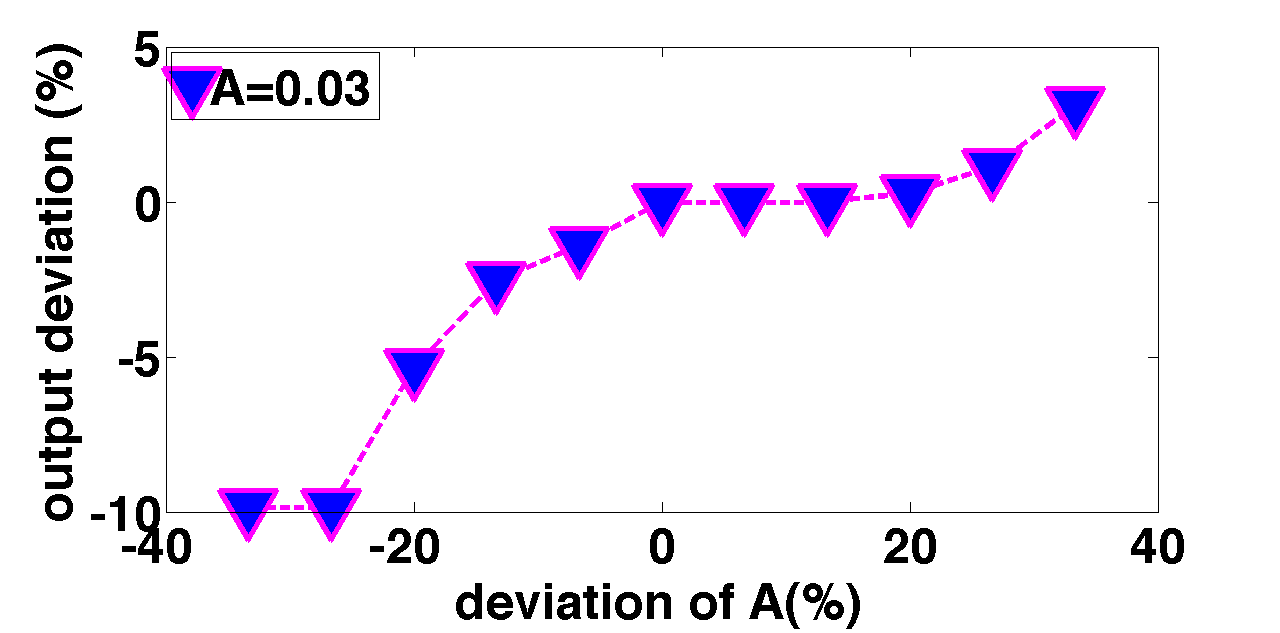
\includegraphics[width=1.55in,height=1in] {figures/sensibility1.png}
		\label{fig:sensibility1}
	}
	\subfigure[subgraph]{
		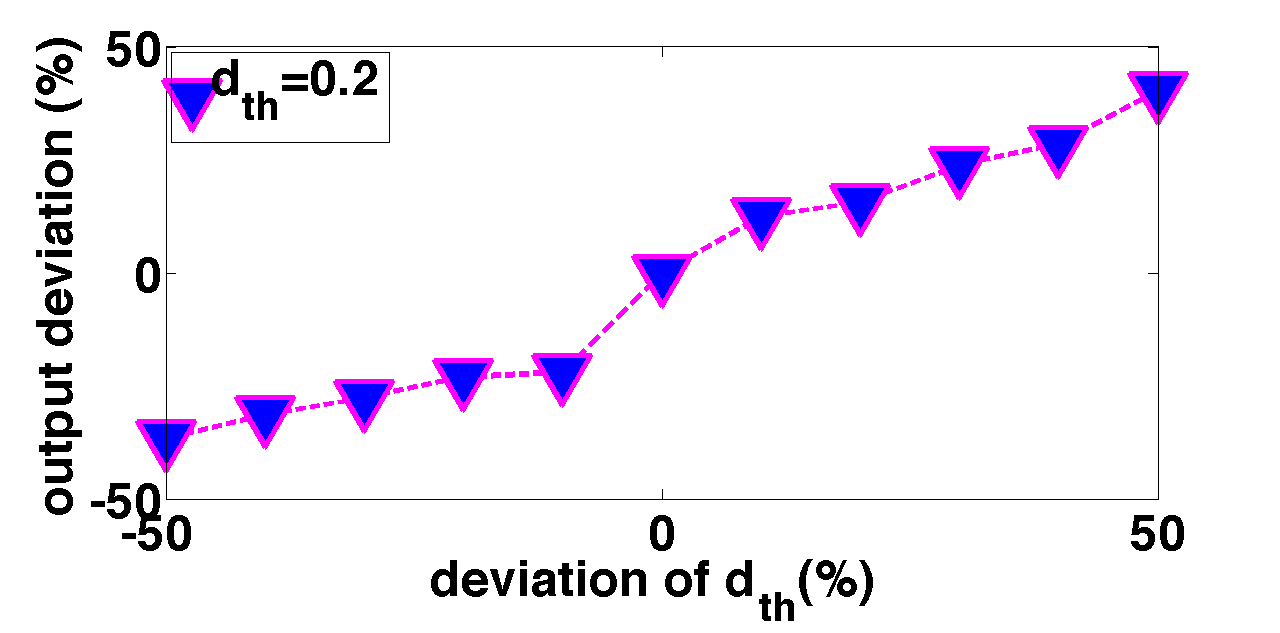
\includegraphics[width=1.55in,height=1in] {figures/sensibility2.png}
		\label{fig:sensibility2}
	}
	\vspace{-1em}
	\caption{Sensibility comparison of the two algorithms.}
	\label{fig:sensibility}
\end{figure}

\subsection{Absenteeism case study}
\subsubsection{What caused absenteeism?}
To retrospect what caused the group absenteeism is never a trivial task,  because there are so many factors that might affect whether people post Tweets or not, and how frequent they post Tweets. Generally, the absenteeism of Tweets can be explained at leaf of the two aspects.

\paragraph{Population mobility}
The population at one location is not a constant, which can vary at different time. As shown in Fig~\ref{fig:holidays_brazil}, We plot the Tweets of 131 cities in Brazil based on the weekdays and holidays from June 2013 to May 2014. From Figure~\ref{fig:holidays_brazil}, we can see that usually Friday features the lowest Tweets volume, and holiday also has a low Tweets volume, but has the highest deviations. Take the example of Chetumal, Quintana Roo, Mexico on May 1st, whose absenteeism score is $-3.00$. For the day of May 1st, which happens to be Labor Day of Mexico, large amount of people go out for travel, resulting in absenteeism in the local town.
%\begin{figure}[h]
%	\centering
%	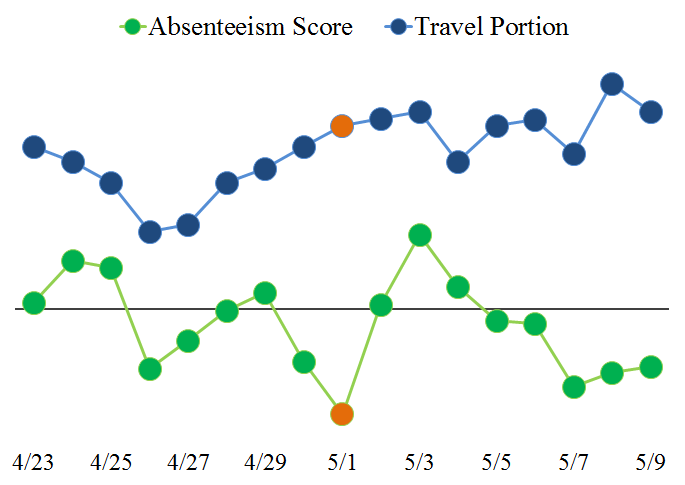
\includegraphics[width=1.8in, height=1in]{figures/userid_portion.png}
%	\caption{Absenteeism score correlate with people's travel portion, in Chetumal, Quintana Roo, Mexico, from Apr-23-2014 to May-09-2014. The orange circle shows on May-01-2014 (the national holiday), the deepest absenteeism score corresponding to a higher travel portion.
%	}
%	\label{fig:userid}
%\end{figure}

\begin{figure}[h]
	\centering
	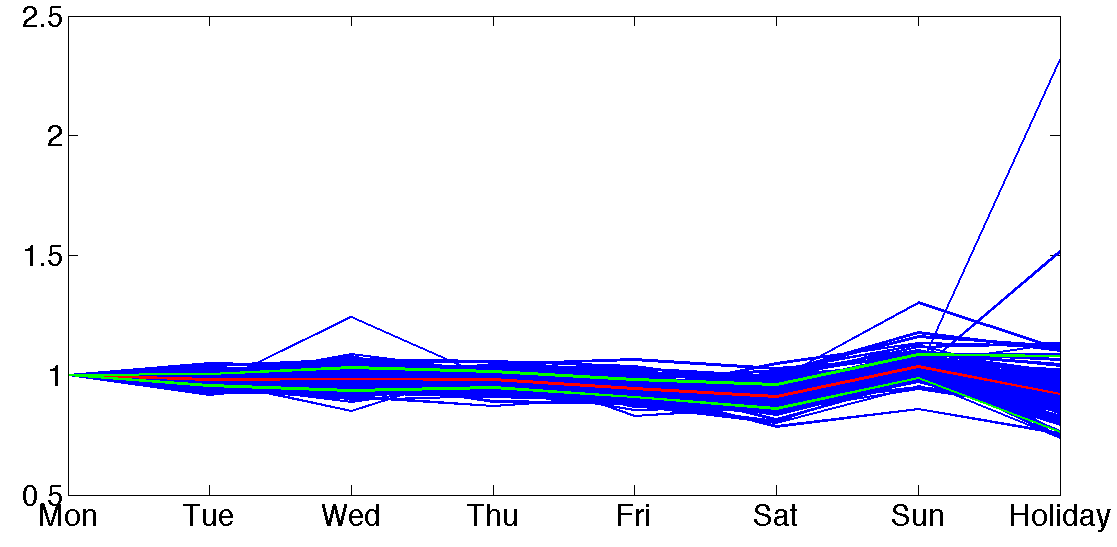
\includegraphics[width=2in]{figures/HolidayCurve_Brazil.png}
	\caption{Tweets daily volume of 131 cities from June 2013 to May 2014. Each day's volume is normalized by Monday's average value. The red line represents the $mean$ value, and the green lines represent the $mean\pm \sigma$ boundaries.
	}
	\label{fig:holidays_brazil}
\end{figure}

\paragraph{Major (negative) events}
Tweets rate is heavily depends on people's social activities, especially when major negative events happen. For instance, at 15PM on Sep 11, 2013, Mexico, a large portion of people were involved in protest that they have no time to Tweet, which results in Twitter absenteeism from 15:00 to 15:30. Tweets rate is also closely depends on people's sentiment, for instance, on Jan 31, 2014, Chile'S IPSA stock index hit lows not seen in over 4 year, people might not like to Tweet. Even weather has a close relationship with the Tweets number. Usually, a good weather introduces more topic for people. Otherwise, severe weather like heavily storms which result in floods usually hinder people from doing any entertainment, and the Tweets number will drop down, as shown in table~\ref{table:list_events}.

\subsubsection{Why use group absenteeism?}
\paragraph{Irreplaceable}The unique of absenteeism signal made it plays a special role in event detection. For instance, on May 16, 2014, when the anti-World cup protest happened on cities Rio de Janeiro and Sao Paulo, large portion of people walked on the street for protest, both cities' Tweets absenteeism score reach the lowest point, see Figure~\ref{fig:World_cup}. Also the case of Brazil floods on Dec 12, 2013 is the same situation, when heavy rains caused floods, while the floods get more and more severe, the Tweets tends to be inactive, and on the day of Dec 24, the floods was the worst day, while at the same time, the Twitter at local state reached the lowest absenteeism score, see Figure~\ref{fig:Brazil_flood}. In the two cases, using burst algorithm cannot identify such events by only observing Twitter burst activity.

\begin{figure}[h]
	\centering
	\subfigure[]{
		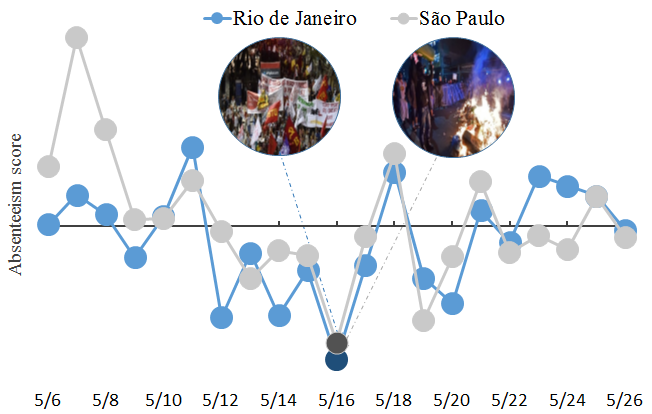
\includegraphics[width=1.55in,height=1in] {figures/Worlp_cup_example1.png}
		\label{fig:World_cup}
	}
	\subfigure[]{
		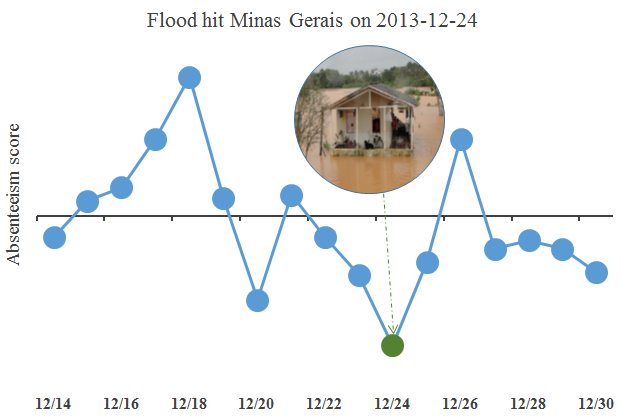
\includegraphics[width=1.55in,height=1in] {figures/flood_example.png}
		\label{fig:Brazil_flood}
	}
	\vspace{-1em}
	\caption{ (a) Tweets Absenteeism score in two cities of Brazil while they are proceeding anti-world cup protest on May-16-2014. (b) Tweets Absenteeism score reach the lowest point when floods hit Minas Gerais, Brazil on Dec-24-2013.}
	\label{fig:flood_cup}
\end{figure}

\paragraph{Earlier signal}
Take the case of Apr 01, 2014 Chile earthquake for instance, when the earthquake erupted at 20:46 local time, the Twitter appears a strong group absenteeism signal at the very first 4 minutes, after that, Twitter started to burst. Using the subgraph algorithm, when the time window set enough small, it can capture the group absenteeism much earlier than the later burst signal. We can see using very small-grained time interval, employing the absenteeism algorithm is able to capture the abnormal Twitter activity earlier, especially when facing emergence events.
\begin{figure}[h]
	\centering
	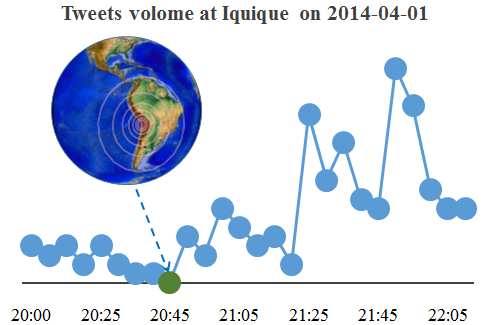
\includegraphics[width=1.8in, height=1.1in]{figures/earthquake_example.png}
	\caption{Tweets volume at Iquique, Tarapacá, Chile on Apr-01-2014. After the M8.2 earthquake erupt, in 4 minutes, the geocoded Tweets at Iquique is 0.
	}
	\label{fig:earthquake}
\end{figure}


% % % % % % % % % % % % % the end% % % % % % % %
%
%\subsubsection{What caused absenteeism?}
%To retrospect what caused the group absenteeism is never a trivial task,  because there are so many factors that might affect whether people post Tweets or not, and how frequent they post Tweets. For simplicity, we model the Tweets volume of city $c$ on day $d$ as the following function:
%\begin{equation}
%  \label{eq:3D_distance}
%  \begin{array}{l}
% 	\mathcal{TW}(c,d) = \mathcal{M}*\beta
%  \end{array}
%\end{equation}
%$\mathcal{M}$ is the Twitter user number, and $\beta$ is the average Tweets number that one user post in time unit. According to this mechanism, the absenteeism of Tweets can be explained at leaf of the two aspects.
%
%\paragraph{User number $\mathcal{M}$}
%Usually, $\mathcal{M}$ is not constant, and varies at different time. As shown in Fig~\ref{fig:holidays_brazil}, We plot the Tweets of 131 cities in Brazil based on the weekdays and holidays from June 2013 to May 2014. From Figure~\ref{fig:holidays_brazil}, we can see that usually Friday features the lowest Tweets volume, and holiday also has a low Tweets volume, but has the highest deviations. Take the example of Chetumal, Quintana Roo, Mexico on May 1st, whose absenteeism score is $-3.00$. For the first event day is May 1st, which happens to be Labor Day of Mexico, large amount of people go out for travel, resulting in absenteeism in the local town.
%\paragraph{Tweets rate $\beta$}
%Tweets rate is heavily depends on people's social activities. For instance, at 15PM on Sep-11-2013, Mexico, a large portion of people were involved in protest that they have no time to Tweet, which results in Twitter absenteeism during this time slot. Tweets rate is also closely depends on people's sentiment, for instance, on Jan-31-2014, Chile'S IPSA stock index hit lows not seen in over 4 year, people might not like to Tweet. Even weather has a close relationship with the Tweets number. Usually, a good weather introduces more topic for people. Otherwise, severe weather like heavily storms which result in floods usually hinder people from doing any entertainment, and the Tweets number will drop down, as shown in table~\ref{table:list_events}. 

\section{Conclusion} \label{sec:conclusion}
In this paper, we disclose an interesting inactive behavior, group absenteeism in Twitter. We study the group absenteeism phenomena in south American, and propose two group absenteeism approaches: regional group absenteeism and subgraph group absenteeism. The experiment results show that both approach help people to detect some potential social events, such as pandemic, migration of population, and natural disaster. In the future work, we are going to invest the deeper mechanism of the group absenteeism in social network.



%\begin{thebibliography}{99}
%\bibliography{sigproc}

\bibliographystyle{IEEEtran}
\bibliography{sigproc}

%\end{thebibliography}
\end{document}

% End of ltexpprt.tex
%


